\documentclass[conference]{IEEEtran}
\IEEEoverridecommandlockouts
% The preceding line is only needed to identify funding in the first footnote. If that is unneeded, please comment it out.
\usepackage{cite}
\usepackage{amsmath,amssymb,amsfonts}
\usepackage{algorithmic}
\usepackage{graphicx}
\usepackage{textcomp}
\usepackage{xcolor}
\usepackage{float}
\def\BibTeX{{\rm B\kern-.05em{\sc i\kern-.025em b}\kern-.08em
    T\kern-.1667em\lower.7ex\hbox{E}\kern-.125emX}}
\begin{document}

\title{HOMEWOEK 1}

\author{\IEEEauthorblockN{Runlin Hou}
\IEEEauthorblockA{\textit{ECE, School Of Graduate Studies} \\
\textit{Rutgers University}\\
hourunlinxa@gmail.com}
}

\maketitle

\section*{Question I}

In this problem, we are supposed to solve the 3-sum problem with two different methods
whose orders are $O(N^3)$ and $O(N^2logN)$.
The purpose of the 3-sum problem is to find the amount of triples sum to exactly zero in 
a given list.

\subsection*{Implementation}

The easiest solution is to use a three-layer traversal for a single triple. This method can
be seen that we have three pointers. We will fix the first two pointers so that we can find 
the third pointer that make the three values sum to zero by one traversal. Since each pointer
are supposed to traverse the whole list to exhaust all combinations, the order of this 
solution would be $O(N^3)$.

Based on the first solution, we want to make some improvement. The basic idea of the firt 
solution is to find third value make the three numbers sum to zero. So we are actually 
dealing with a seeking problem on the third pointer. And the way we solve it, traversal, 
provides an order $O(N^3)$. But there is a better way. As we all known, binary search can 
provides an order $O(logN)$ to find a specific number on a sorted sequence which is obviously
better than $O(N)$. So the improved solution can be achieved by replacing the traversal to 
binary search on the third pointer. 

Since we are going to sort the list before we do the binary search. We are supposed consider 
the time consumption of the sort algorithm. I look up the sort function contained in the list 
class in Python. \verb|list.sort()| is based on the timesort algorithm whose order is $NlogN$.
So it is obvious that this sorting process will not extend the order of the whole algorithm.

However, if we are going to use bianry search to locate the third pointer, we may face a 
situation that couple entries share a same value. For example, we may have a list look 
like this \verb|[-1,-1,0,1,1]|. To explain this easier, let's represent the five number by 
\verb|[a1,a2,a3,a4,a5]|. As we known binary search will find \verb|a4| is a suitable answer
when the first two pointer points to \verb|a1| and \verb|a3| since $-1+0+1=0$. But here comes
the problem, binary search will stop after it find the first 1, which is represented by \verb|a4|
As thus, another suitable triple \verb|a1,a3,a5| would be ignored. The traversal solution won't
face this problem because the traversal won't stop until the last enrty of the list, so that 
it can return multiple answers in a single traversal. To avoid this in binary search, we need
to find how many same values we have in the rest of the list, which is also easy to solve since
the list is already sorted.

\subsection*{Performance}
We run the two algorithm on the 7 datasets with 8, 32, 128, 512, 1024, 4096, 8192 entries. 
And get the data as following:

\begin{table}[H]
    \caption{Time consumption for 2 algorithm}
    \begin{center}
        \begin{tabular}{|c|c|c|}
            \hline
             & Q1-1 $O(N^3)$ & Q2-2 $O(N^2logN)$\\
            \hline
            8&	0.0013&	0.0000 \\
            \hline
            32&	0.0030&	0.0010 \\
            \hline
            128&	0.0490&	0.0180 \\
            \hline
            512	&2.1775&	0.4434 \\
            \hline
            1024&	17.1487&	2.0825 \\
            \hline
            4096&	1070.0717&	39.5941 \\
            \hline
            8192&	8529.9315&	175.7147 \\       
            \hline
            \multicolumn{3}{l}{recorded in seconds}\\
        \end{tabular}
    \end{center}
\end{table}

\begin{figure}[H]
    \centerline{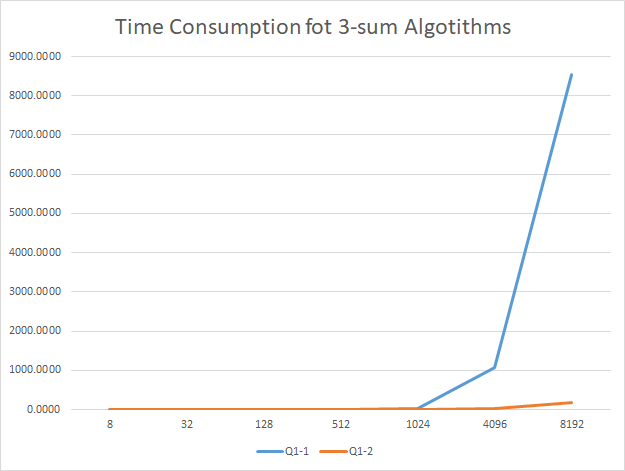
\includegraphics[scale=0.5]{Pic/fig1.png}}
    \caption{Time consumption for 2 algorithm}
\end{figure}

As we can see in the above graph, the time consumption of the fisrt algorithm is obviously 
larger than the second one. When it cames to the dataset with 8192 entries, the time consumption
of the first algorithm is more than 40 time compared to the second one. 

For the fisrt algorithm, 
we can see that the time consumption growth roughly obey $N^3$, if we see the last three rows.
8192 is 8 times of 1024, so that the time consumption is about $8^3=512$ times larger. 8192 is 
2 times of 4096, so that time consumption is $2^3=8$ times. 

For the second algorithm, the growth of the time consumption roughly obey $N^2logN$. Similarly,
we can also check for the last three rows. If we take the time consumption of 1024 entries as
a standard, we can get the rest two results should be around $16\frac{12}{10}\times 2.08=39.936$
and $64\frac{13}{10}\times 2.08=173.056$. We can see that the they are really close to the real
results.

\section*{Question 2}
Unio-Find problem require us to make a judgment of the connection of 
two points. And we have three solutions for this problem.

\subsection*{Implementation}
The three solutions can be seen as two solutions and the third solution
is actually a improvement based on the second solution.

The first way is the easiest to figure out. Since we have 8192 points
total, we will initialize a id set with all the 8192 points. The basic
idea is to set the two points to have the same id when they were 
connected. This is the Union Process. Since the points connected 
together share the same id. It would be easy for us to make the 
judgment \verb|id[a] == id [b]|. So the order of union part would be $O(N)$ 
cause we have to do a traversal to set all the connected points to have
the same id, which also provide an advantage that the order of judgment
process is $O(1)$.

The second solution based on the tree struction. Still, we need to initialize an id
list. But during the union process, we will not set the connected points to have
the same id. Instead, we introduce a new attribute root. When two points are 
connected together, one of the points' id would be set to be the root of the these
two points and these two points can be called a tree. And when two points that 
already in a tree are connected together, we will seek back to their roots and 
set one the two roots to be the root of the new tree who is the combination of these
two trees. By this method we my reduce the order to $log(N)$, if we are locky enough
to get a well placed tree.

The third method is basicly the same with the second one. To make sure we have a 
lower tree so that we can same a lot of time for seeking the root. We will add the
smaller tree to the bigger tree, so that the hight of the trees will always be the 
smallest.
By this method, we can reduce the order to $log(N)$, meanwhile this
also bring us a disadvantage that we increase the order of judgment to $log(N)$ 
either. Cause we need to find the root of the tree to see if these two points are 
connected. 

\subsection*{Performance}

\begin{table}[H]
    \caption{Time Consumption}
    \begin{center}
        \begin{tabular}{|c|c|c|c|}
            \hline
             & QF $O(M*N)$ & QU $O(M*N)$ & WQU $O(M*logN)$\\
            \hline
            8	&0.003149&	0.000002&	0.000002\\
            \hline
            32	&0.012309&	0.000007&	0.000007\\
            \hline
            128	&0.049540&	0.000028&	0.000027\\
            \hline
            512	&0.200586&	0.000122&	0.000108\\
            \hline
            1024&	0.385200&	0.000217&	0.000215\\
            \hline
            4096&	1.545487&	0.000871&	0.000859\\
            \hline
            8192&	2.694597&	0.001694&	0.001621\\
            \hline
            \multicolumn{3}{l}{recorded in seconds}\\
        \end{tabular}
    \end{center}
\end{table}

\begin{figure}[H]
    \centerline{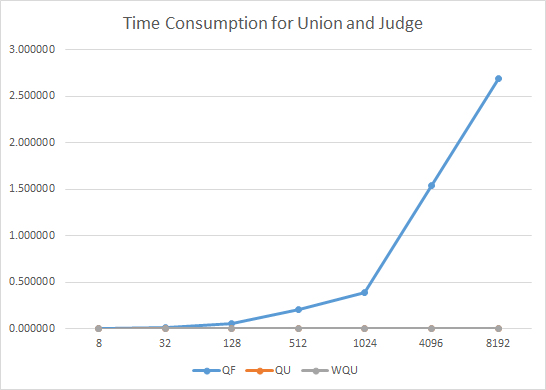
\includegraphics[scale=0.5]{Pic/fig2.png}}
    \caption{Time consumption for 3 Union and Judge}
\end{figure}

For the execution of union and judgment, we can see that the fisrt method
takes the longest time, which is what we expected. 

\begin{figure}[H]
    \centerline{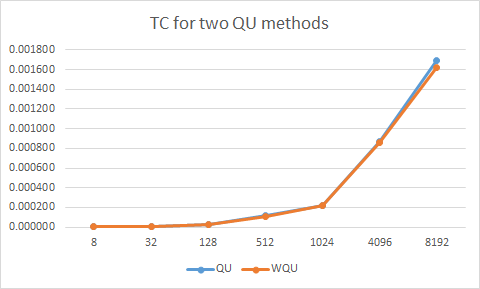
\includegraphics[scale=0.5]{Pic/fig3.png}}
    \caption{Time consumption for 2 Union and Judge}
\end{figure}

To see the two Quick Union perfoemance better, I plot them in a new graph. As the
graph shown, these two methods didn't show an obvious improvement, which is not 
what we expected, since the order of two methods are supposed to be $O(MN)$ and 
$(MlogN)$. I think the problem is that this two algorithm happened to create two similar tree
so the time for searching and union are basicly the same.

\section*{Question 3}
To get $N_c$, the general thought is to estimate the $f(N)$ according to the 
data we have and set $C$ to be proper value. By talking to my friends,  I decide 
to use a Python function \verb|spicy.curve_fit| as a tool to get the estimate function.
This function use dichtomy to fit a dataset to an assumed function.
\subsection*{Q1-1}
We assume the function $f(N)$ and use curve\_fit:
\[\begin{aligned}
    f(N)=&aN^3+bN^2+cN+d\\
    f(N)=&1.54622457e-08N^3+4.30171955e-07N^2\\
    &7.44238753e-05N-6.14828498e-03
\end{aligned}\]
Now we set $C=1$, since $g(N)=N^3$, it is easy to see whenever $N>1$, we get $f(N)<N^3$. So $N_c=1$.
\subsection*{Q1-2}
We assume the function $f(N)$ and $g(N)=N^2logN$, use curve\_fit:
\[\begin{aligned}
    f(N)=&aN^2logN+bNlogN+clogN+d\\
    f(N)=&2.06804564e-07N^2logN\\
    &-4.80720006e-05NlogN\\
    &+4.63993636e-02logN+1.95971843
\end{aligned}]\]
For this case, the sum of the coefficients is a little bit larger than 2.
\[\begin{aligned}
    &\frac{f(N)}{g(N)}<\frac{cg(N)}{g(N)}=c\\
    &C=\frac{2.005N^2logN}{N^2logN}=3
\end{aligned}\]
So when we set $C=3$, $N_c$ would still be 1.

Now if we set $C=1$, $N_c$ would be 2 since $g(2)=4>f(2)$

\subsection*{Q2-1}
We assume the function $f(N)$ and $g(N)=N^2$, use curve\_fit:
\[\begin{aligned}
    f(N)=&aN^2+bN+c\\
    f(N)=&-1.12744082e-08N^2+4.22707330e-04N\\
    &-8.98749604e-03
\end{aligned}\]
Now we set $C=1$, also we can get whenever $N>1$, $f(N)<N^2$. So $Nc=1$.
\subsection*{Q2-2}
We assume the function $f(N)$ and $g(N)=N^2$, use curve\_fit:
\[\begin{aligned}
    f(N)=&aN^2+bN+c\\
    f(N)=&-1.35496123e-12N^2+2.17718643e-07N\\
    &1.44896813e-06
\end{aligned}\]
Now we set $C=1$, also we can get whenever $N>1$, $f(N)<N^2$. So $Nc=1$.
\subsection*{Q2-3}
We assume the function $f(N)$ and $g(N)=NlogN$, use curve\_fit:
\[\begin{aligned}
    f(N)=&aNlogN+blogN+c\\
    f(N)=&-2.75991000e-12NlogN\\
    &-2.20840089e-07logN\\
    &-2.25868736e-06
\end{aligned}]\]



\section*{Question 4}
For this problem, we are actually finding the largest value and the smallest value in the 
sequence. My thought is to set to pointers who point to the max and the min value we've 
already met. And we will compare every new entry with these two values. Every time we met a 
value larger than the max or smaller than the min, we update the pointer. So that we can 
find the max and the min value in a single traversal. And the order of this algorithm would 
be $O(N)$, cause the whole process will finish in one traversal.

\begin{table}[H]
    \caption{Time Consumption}
    \begin{center}
        \begin{tabular}{|c|c|}
            \hline
             & Fathest Pair $O(N)$\\
            \hline
            8	&0.0000041\\
            \hline
            32	&0.0000056\\
            \hline
            128	&0.0000135\\
            \hline
            512	&0.0000407\\
            \hline
            1024&	0.0000985\\
            \hline
            4096&	0.0003100\\
            \hline
            8192&	0.0006266\\
            \hline
            \multicolumn{2}{l}{recorded in seconds}\\
        \end{tabular}
    \end{center}
\end{table}

\begin{figure}[H]
    \centerline{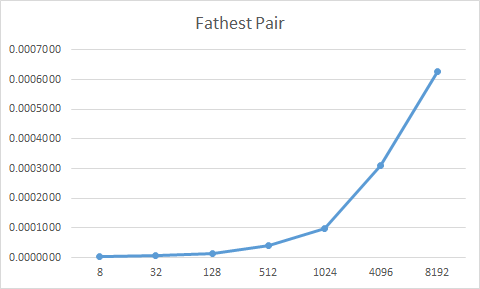
\includegraphics[scale=0.5]{Pic/fig4.png}}
    \caption{Time consumption for Fathest Pair}
\end{figure}

We can see that the time consumption fits our expectation, it shows a linear growth.

\section*{Faster 3-sum}
As we mentioned in the Question 1, 3-sum aims at finding a triple that sums to zero.
The idea of the first two methods in Question 1 is to fix the first two value and try 
to find if there exists a value make the triple sum to zero. By this way, it is hard to 
reduce the order smaller than $O(N^2)$, cause they require a 2-layer traversal to make
sure we hit every 2- value combinations. 
But if we fix only one value and try to find a couple that sums to be its negative. 
On a sorted sequence, we set two pointers at the head and the tail. Since the sequence
has already been sorted, we move head pointer to right will definitely make the sum 
greater and also moving the tail left will definitely make the sum smaller. Based on this
method we can find a couple in a single traversal. And combined this with the fixed value,
we can find a triple sums to zero with a algorithm whose order is $O(N^2)$ in the worst case.

\begin{table}[H]
    \caption{Time Consumption}
    \begin{center}
        \begin{tabular}{|c|c|}
            \hline
             & Faster 3-sum $O(N)$\\
            \hline
            8	&0.0000\\
            \hline
            32	&0.0001\\
            \hline
            128	&0.0019\\
            \hline
            512	&0.0282\\
            \hline
            1024&	0.1142\\
            \hline
            4096&	1.8214\\
            \hline
            8192&	7.2870\\
            \hline
            \multicolumn{2}{l}{recorded in seconds}\\
        \end{tabular}
    \end{center}
\end{table}

\begin{figure}[H]
    \centerline{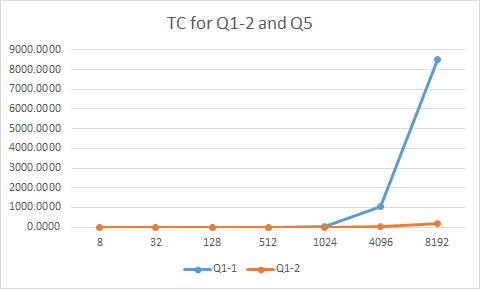
\includegraphics[scale=0.5]{Pic/fig5.png}}
    \caption{Time consumption for Q1-2 and Q5}
\end{figure}

As we can see the time consumption shows a qudratic growth.
\end{document}
